\section{Dataset}
% Delete the text and write your Results here:
%------------------------------------
\subsection{Dataset Used}
To ensure fairness in the improvement of our model, we opted to use the same computerized block diagram that was presented by the authors. This new dataset comprised of 502 diagrams and contained more than 13,000 annotated elements (shapes, edges, and text phrases) and was retrieved on GitHub. There are total 7 classes, each for a block element: Connection for circle, Data for parallelogram, Decision for diamond, Terminator for eclipse, Arrow, Text and Process for all other shapes not mentioned above. 

\subsection{Data Augmentation}
As highlighted previously, a key limiting factor that mitigated the performance of the original Inception-ResNet-v2 model was the difficulty of obtaining useful annotated data sets for object detection models. Despite scraping 502 images online, the manual task of annotating them with detailed labels (shapes, arrows, texts), bounding-boxes, and creating human-written summaries is labour-intensive and time-consuming. 

Additionally, the 502 images had limited variability as shown in Figure~\ref{fig: Class Instances of the CBD Dataset}. The dataset would not capture the full diversity of block diagrams, including different shapes, shape representations, text styles, and arrow connections. In this work, we propose to a data generation plan with an existing knowledge base and Mermaid graphing tool. With an additional new dataset, it would be able to help improve the generalization capabilities of our model compared to other datasets. 

\begin{figure}
    \centering
    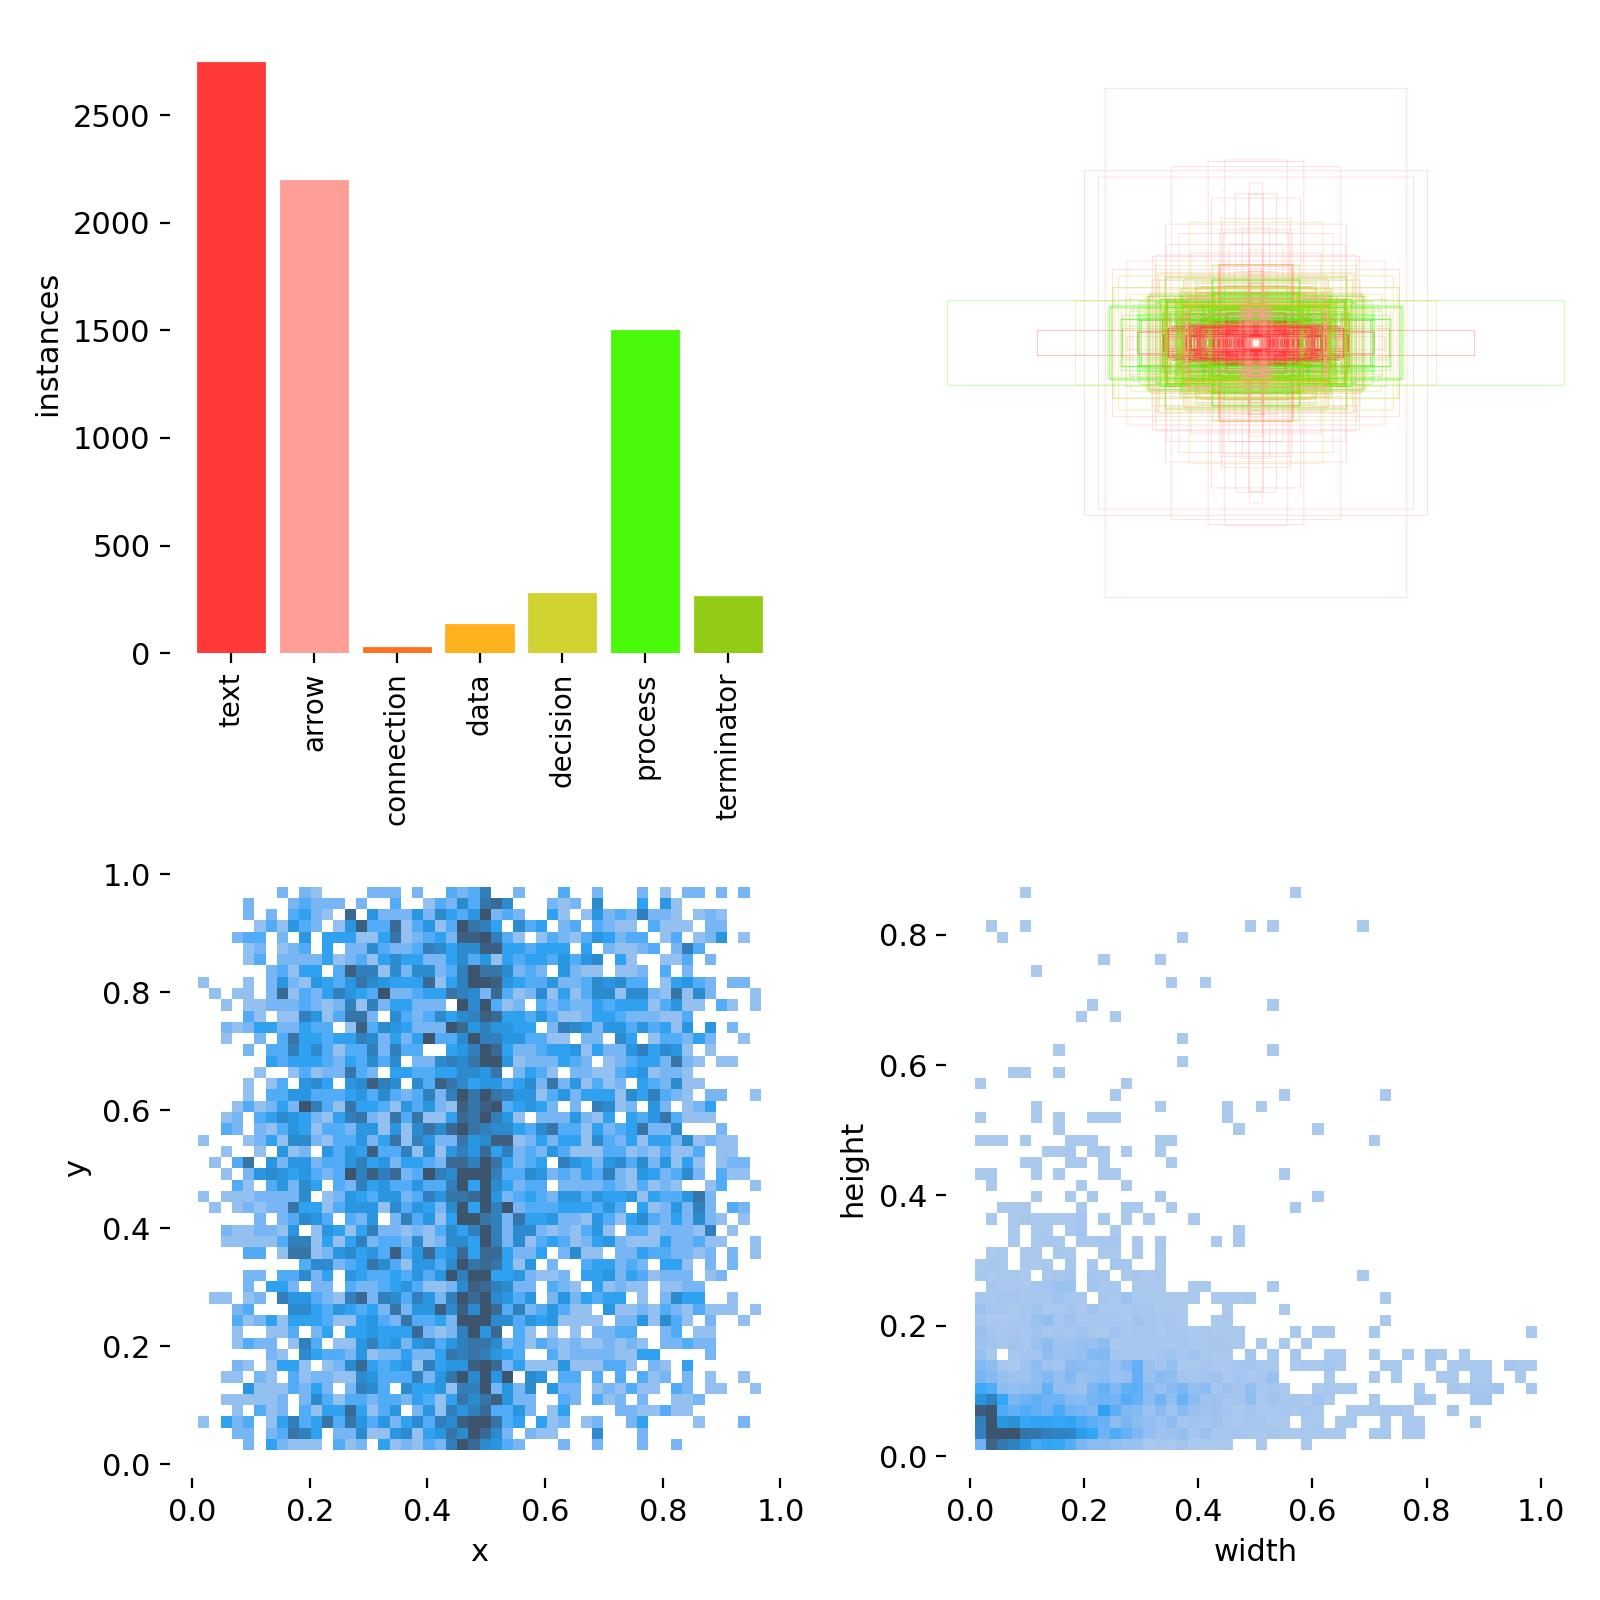
\includegraphics[width=0.48\textwidth]{Images/Class Representation.jpg}
    \caption{Class Instances of the CBD Dataset}
    \label{fig: Class Instances of the CBD Dataset}
\end{figure}


This ideally allows models to learn how to reverse engineer the entity-relation-entity triplets from the generated diagrams. For each entity-relation-entity triplet $x=[e_{1}, r, e_{2}]$, construct a directed graph $G = (V,E)$ such that there exists vertices $e_1,e_2 \in V$, a directed edge $(e_1,e_2) \in E$ with label $r$ for all $x \in X$, where $X$ represents set of all triplets in the knowledge graph. An pseudo-code version of this algorithm is shown in Figure~\ref{fig: Pseudo-code for the graph generation algorithm}. Finally, visualize this graph using certain visualization tools such as Mermaid, and easily obtain the labels and bounding-boxes for the diagram because of it's computerized nature.

\begin{figure}
    \centering
    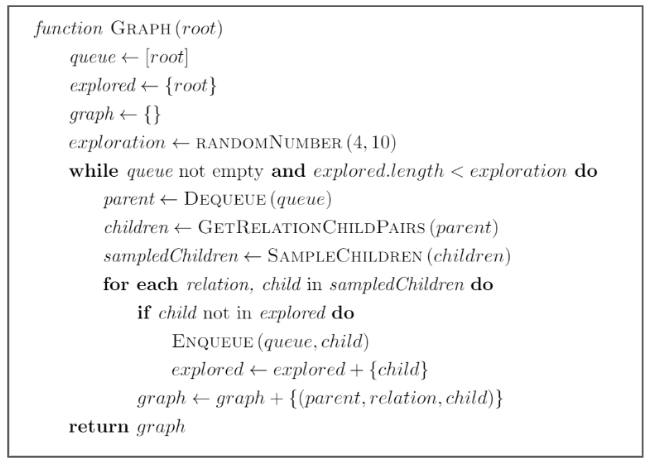
\includegraphics[width=0.48\textwidth]{Images/Graph generation algo.png}
    \caption{Pseudo-code for the graph generation algorithm}
    \label{fig: Pseudo-code for the graph generation algorithm}
\end{figure}




